\documentclass[printMode=false, declarePage=false]{ecnuthesis}
% 
% 本模板源代码托管在
% https://github.com/Koyamin/ECNUThesis-Undergraduate
% 最新的 Release 版本将发布在该仓库
% 
\ecnuSetup{
  info = {
    title = {重中性轻子的唯象学特性与 {NGC 1068} 多信使观测研究},
    % 中文标题
    %
    titleEN = {Research on Phenomenology of HNL and Multi-Messenger Observation of NGC 1068},
    % 英文标题
    %
    author = {韦晾},
    % 作者姓名
    %
    studentID = {10224511412},
    % 作者学号
    %
    department = {物理学院},
    % 学院名称
    %
    major = {物理学},
    % 专业名称
    %
    supervisor = {阮建红},
    % 指导教师姓名
    %
    academicTitle = {教授},
    % 指导教师职称
    %
    year  = 2026,
    % 论文完成年份
    %
    month = 4,
    % 论文完成月份
    %
    graduationYear = 2026,
    % 内封面毕业届别
    % 说明:
    %   若 graduationYear 字段为空，则内封面毕业届别为 year
    %
    keywords = {重中性轻子, 逆翘翘板机制, NGC 1068, 多信使},
    % 中文关键词
    % 请使用英文逗号 "," 以分隔
    %
    keywordsEN = {HNL, ISS, NGC 1068, multi-messenger},
  },
  style = {
    numbering = arabic,
    % 章节编号样式
    % 可用选项:
    %   numbering = arabic|alpha|chinese
    % 说明:
    %   arabic    使用数字进行编号 (即理科要求)
    %   alpha     使用字母进行编号 (即外文要求)
    %   chinese   使用汉字进行编号 (即文科要求)
    %   (默认选项为 arabic )
    %
    font = times,
    % 西文字体选择
    % 可用选项:
    %   font = lm|times|xits
    % 说明:
    %   lm        使用 TeX 自带的 Latin Modern 字体
    %   lm        使用 TeX 自带的 XITS 系列字体
    %   times     使用 Times 风格的西文字体
    %   (默认选项为 xits )
    %
    fontCJK = fandol,
    % 中文字体选择
    % 可用选项:
    %   fontCJK = fandol|windows|mac
    % 说明:
    %   fandol    使用 TeX 自带的 fandol 字体
    %   windows   使用 Windows 系统内的字体 (中易)
    %   mac       使用 MacOS 系统内的字体
    %   (默认选项为 fandol )
    %
    logoResource = {./ecnu-vi-inner-cover-logo.pdf},
    % 封面插图数据源
    % 模版已自带, 位于 ./source/inner-cover(contains_font).eps
    % 默认值为空
    %
    % declarePageResource = {./source/declaration.pdf},
    % 扫描版声明页 PDF 文件
    % 若该值为空则生成模版预定义的声明页；否则将插入指定路径所对应的 PDF 文件
    % 默认值为空
    %
    bibResource = {./ref.bib}
    % 参考文献数据源
    % 由于使用的是 biber + biblatex , 所以必须明确给出 .bib 后缀名
    %
  }
}

\usepackage{enumitem}
\usepackage{mwe}
\usepackage{tikz-feynman}
\usepackage{siunitx}
\usepackage{slashed}

\begin{document}

% 目录
\tableofcontents

% 声明前置部分开始, 页码设置为大写罗马数字
\frontmatter

\begin{abstract}
  随着多信使天文学的发展，IceCube 探测器在近期确认了活动星系核（AGN）NGC 1068 作为高能中微子点源。然而，结合现
  有的 $\gamma$ 射线观测数据，传统的电磁级联模型在解释其核心区域的遮蔽现象时存在一定困难。本文基于重中性轻子（HNL）
  模型，探讨了其作为解释这一多信使观测结果潜在机制的可能性。
  本文首先通过 Inverse Seesaw （ISS）机制引入HNL，详细计算了在AGN高能环境中，不同质量的 HNL 通过$\pi$介子和$\mu$子衰变的产生时，
  相比较于产生标准模型中微子的分支比，以及产生的 HNL 粒子在母粒子静止系下的螺旋度分布、不同螺旋度的 HNL 粒子在轻子衰变与辐射衰变通道中产物的能谱分布。
  随后，将该理论模型应用于 NGC 1068 的实际观测数据中，估算了 HNL 输运并转化
  为$\gamma$射线的过程。研究结果表明，如果HNL仅通过ISS机制的轻子衰变产生次级电子并经逆康普顿散射转化为 $\gamma$ 射线，
  其通量远低于现有探测阈值；但若 HNL 存在占主导的偶极辐射衰变通道，则能够部分解释观测到的 $\gamma$ 射线信号，并由此可
  以对 HNL 与 $\nu_\mu$ 的混合角 $|U_\mu|^2$ 给出相应的参数空间上限限制。
\end{abstract}

\begin{abstractEN}
  With the advance of multimessenger astronomy, the IceCube detector has recently identified the active galactic nucleus
  (AGN) NGC 1068 as a source of high-energy neutrinos. However, when combined with existing γ-ray observations, conventional
  electromagnetic cascade models encounter difficulties in explaining the attenuation observed in its core region. In 
  this work we investigate the heavy neutral lepton (HNL) scenario as a potential mechanism to account for these multimessenger 
  observations.
  We first introduce HNLs via the Inverse Seesaw (ISS) mechanism and compute in detail, in the AGN high-energy environment, the 
  production of HNLs from $\pi$ and $\mu$ decays for different HNL masses, comparing their branching ratios to those for 
  standard-model neutrino production. We also calculate the helicity distributions of HNLs produced in the parent particle 
  rest frame, and the energy spectra of decay products from HNLs of different helicities in both leptonic decay and radiative 
  decay channels. We then apply this theoretical framework to the observational data of NGC 1068 to estimate HNL transport and 
  their conversion into $\gamma$ rays. Our results show that if HNLs only produce secondary electrons via ISS-driven leptonic decays which 
  then generate $\gamma$ rays through inverse Compton scattering, the resulting flux is far below current detection thresholds; 
  however, if HNLs possess a dominant dipole radiative decay channel, they can partially account for the observed $\gamma$-ray signal. 
  From this we derive corresponding upper-limit constraints on the HNL-$\nu_\mu$ mixing angle $|U_\mu|^2$.
\end{abstractEN}

% 声明正文部分开始, 页码设置为阿拉伯数字
\mainmatter

\chapter{引言}

\section{背景}

随着天文观测技术的不断进步，更多的信号被纳入到天文观测的对象中。除了传统的可见光，无线电波等各种波段的电磁波
之外，引力波的探测技术正逐渐成熟，而在宇宙粒子当中，与各种电磁波同样具有探测遥远星体价值的中微子信号也随着 IceCube
等探测器的运行积累了大量的数据。而中微子作为标准模型中的“异类”，其质量起源和相互作用模式都是研究超越标准模型物理
（BSM）的重要窗口。其中影响最大的观测之一是 IceCube 近期确认的高能中微子点源 \cite{icecube2022evidence}。而类似
IceCube 的探测器也有许多正在建设当中，如 KM3NeT/ARCA 探测器，其探测能力覆盖了从 TeV 起的高能范围，
由于其地理位置，KM3NeT/ARCA 对南天球的观测视野良好，对于研究银河系平面等潜在的中微子源区域尤为重要
\cite{km3net2024astronomy}，其已安装完成的探测器已经探测到能量可能高达 220PeV 的中微子信号
\cite{km3net2025observation}。

在 IceCube 等针对 TeV 高能范围的中微子探测之前，已有如神冈探测器（Kamiokande）等探测站。利用 Kamiokande 人类
首次直接观测到来自太阳系外的中微子，即来自大麦哲伦星系的超新星SN1987A爆发的中微子事件\cite{hirata1988observation}。
其继承者 Super-K 主要研究 MeV 至 GeV 范围内的中微子，最重要的探测成果是证明了中微子振荡的存在，也即证明了中微子存在
质量，为标准模型的完善作出了巨大贡献\cite{fukuda1998evidence}。

地面实验室也存在寻找中微子相关 BSM 模型信号的实验，比如 MiniBooNE 实验 \cite{PhysRevLett.103.241802}
等。虽然这些实验尚未发现
明确的信号，但他们也将可能的参数空间进行了限制 \cite{bryman2019constraints}。然而，来源于天文观测的粒子信号相比
地面实验虽然有通量低等不足，但
大的天文时间和空间尺度，以及极端天体中难以复刻的环境为 BSM 物理的研究提供了潜在的优势。在重中性轻子（HNL）方面，
对于较长寿命的 HNL 粒子，我们可能难以在探测器内观测到其衰变，而在大尺度的天文现象中则不受此限制。

另一方面，在 IceCube 对于活动星系核 NGC 1068 的观测中，与 \parencite{murase2020hidden} 等理
论预测相比对时，可以发现高能
的 $\gamma$ 射线通量尚存在一定量的超出。这说明传统的电磁级联模型只能部分解释 AGN 核心区域的 $\gamma$ 射线遮蔽现
象。一个可能的原因是尽管 AGN 核心（冕区）对高能 $\gamma$ 光子是不透明的，但存在某种转化途径，使能量从核心传播出
来之后再变为可探测的光子信号。一个可能的路径是类轴子粒子（ALP），在文章 \parencite{pant2024constraining} 中有所讨论。
在 NGC 1068 之前，利用对于 SN 1987A 超新星的观测 \cite{PhysRevLett.58.1490}，有对于偶极算符相互作用的 HNL 的
参数空间限制 \cite{Magill_2018}，以及对于轴子和暗光子的研究 \cite{PhysRevD.94.085012} \cite{Chang_2017}。

中微子相关的观测技术的不断发展和成熟开启了多信使天文学更加丰富的时代，同时也为利用天文观测中的中微子信号来寻找
超出标准模型的效应提供了更多的可能性。

\begin{figure}[htbp]
  \centering
  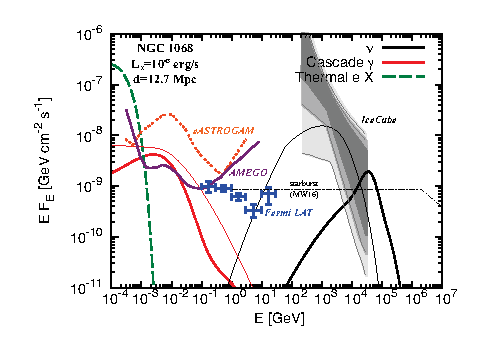
\includegraphics{datas/refplots/NGC1068IC.eps}
  \bicaption{基于 NGC 1068 冕区电磁级联模型的 $\gamma$ 射线通量预测，引用自 \parencite{murase2020hidden}。图中黑线为对于
    中微子通量的不同预测，红色为对 $\gamma$ 射线通量的理论预测。}{Predicted 
    $\gamma$-ray fluxes based on the electromagnetic cascade model for the corona of NGC 1068, taken from \parencite{murase2020hidden}. 
    The black lines represent various predictions for the neutrino flux, while the red lines denote the theoretical predictions for the $\gamma$-ray flux.}
    % 可以看到电磁级联模型良好地解释了较低能量的 $\gamma$ 射线，但对于更高能的部分则低于现有的实验观测。
  \label{fig:spec_theory_predict_gamma}
\end{figure}

\section{本文的主要工作}

在 NGC 1068 的中微子与 $\gamma$ 射线多信使观测结果的解释上，与中微子关系最为密切的重中
性轻子（HNL）也可能存在。在解释中微子质量起源的模型中，如 Type-I Seesaw 和 Inverse Seesaw 模型，都会引入 HNL 粒
子 \cite{king2025righthandedneutrinosseesawmodels}。通过天文观测结果寻找这些粒子的潜在信号，是一个能够发挥天文现
象的尺度优势，与地面实验室结果形成互补的现象学研究。

本文的创新点包括：
计算了 $\pi$ 介子和 $\mu$ 子衰变时产生 HNL 的分支比以及母粒子静止系下，产生的 HNL 螺旋度分布；
计算了考虑自旋的 HNL 轻子和辐射衰变产物的角分布，并进一步推导出不同螺旋度的 HNL
粒子衰变产物的能谱；尝试利用 HNL 解释了 NGC 1068 中的高能 $\gamma$ 射线，讨论了在允许的 HNL 参数空间中的可能性。

本文如此安排：
第二部分讨论 HNL 的理论基础，包括 Type-I Seesaw 机制和 Inverse Seesaw（ISS）机制，从中导出的 HNL 产生与衰变
过程，以及额外的偶极衰变（直接 $\gamma$ 射线衰变）。第三部分讨论 AGN 中产生 HNL 粒子并衰变产生可观测 $\gamma$ 射线信号的可能性，
结合 NGC 1068 的观测数据，尝试解释多信使观测结果，并限制 HNL 的参数空间。最后在第四部分得出结论。

\chapter{HNL 的理论基础}

在探讨 HNL 在天体物理环境中的可观测信号前，本章讨论 HNL 的理论框架。首先，在 2.1 节中我们通过 Inverse Seesaw （ISS）机制
引入 HNL，解释其中微子微小质量的起源及HNL混合角特性。随后，2.2 节详细推导在AGN的高能碰撞环境中，HNL 通过 $\pi$ 介子和 $\mu$ 子
衰变产生的具体途径与运动学特征。最后，2.3节计算HNL的寿命及其主要衰变通道，包括轻子衰变与辐射衰变，
这决定了 HNL 粒子能否逃逸 AGN 的遮蔽区域并产生我们在地球上可观测到的 $\gamma$ 射线。

\section{HNL 起源：ISS 机制}

考虑单代中微子，对标准模型最简单的扩展引入右手中微子场后，允许中微子存在以下的质量项
\begin{equation}
  y_\nu \bar{L} \tilde{H} \nu_R + h.c. \to y_\nu \frac{v}{\sqrt{2}} (\bar{\nu}_L \nu_R + \bar{\nu}_R \nu_L)
\end{equation}
而由于新引入的右手中微子场不参加相互作用，其可以拥有马约拉纳质量项
\begin{equation}
  \frac{1}{2} M_R (\overline{\nu^c_R} \nu_R + \overline{\nu_R} \nu_R^c) 
\end{equation}
定义狄拉克质量为 $m_D = y_\nu \frac{v}{\sqrt{2}}$，可以把中微子质量项写成矩阵的形式，有
\begin{equation}
  \begin{pmatrix}
    \overline{\nu_L} & \overline{\nu_R^c}
  \end{pmatrix}
  \begin{pmatrix}
    0   & m_D  \\
    m_D & M_R
  \end{pmatrix}
  \begin{pmatrix}
    \nu_L^c \\
    \nu_R
  \end{pmatrix}
\end{equation}
这是简化的 Type-I Seesaw 模型 \cite{king2025righthandedneutrinosseesawmodels}。对此矩阵进行对角化之后可以得到中
微子和 HNL 的质量以及混合角为
\begin{equation}
  m_\nu = \frac{m_D^2}{M_R}, \; m_N = M_R, \; |U|^2 = \left( \frac{m_D}{M_R} \right)^2
\end{equation}
一个较大的 $M_R$ 值可以在中微子场与 Higgs 场具有自然的耦合强度时赋予中微子较小的质量。而
Type-I Seesaw 机制中的 HNL 混合角与 HNL 质量耦合，使得在大部分的质量区间，混合角会小得
完全无法探测。如果引入另一费米子场，则可以得到 Inverse Seesaw （ISS）机制，即引入一个带
有马约拉纳质量的费米子场 $S$，矩阵会变为
\begin{equation}
  \begin{pmatrix}
    \overline{\nu_L} & \overline{\nu_R^c} & \overline{S^c}
  \end{pmatrix}
  \begin{pmatrix}
    0   & m_D & 0    \\
    m_D & 0   & M    \\
    0   & M   & \mu
  \end{pmatrix}
  \begin{pmatrix}
    \nu_L^c \\
    \nu_R   \\
    S
  \end{pmatrix}
\end{equation}
在通常的模型中，$M \gg m_D \gg \mu$，$\mu$ 表示了模型中造成轻子数破坏的小量。中微子的
质量和产生的 HNL（在此情况下是一赝狄拉克费米子对，而把其作为狄拉克费米子处理并不影响我们
下文的估算）的质量及混合角为 \cite{king2025righthandedneutrinosseesawmodels}
\begin{equation}
  m_\nu = \mu \frac{m_D^2}{M^2}, \; m_N = M, \; |U|^2 = \frac{m_\nu}{\mu}
\end{equation}
引入 ISS 机制后，由于多引入了一个表示轻子数破坏的 $\mu$ 参数，使得混合角与 HNL 粒子的质量解耦。
因此可以在自然地赋予中微子微小质量的同时，产生可观测的 HNL 混合角与质量。

\section{HNL 的产生途径}

\subsection{$\pi^\pm$ 衰变}
AGN 环境中通过 $p - p$ 与 $p - \gamma$ 过程产生大量的 $\pi$ 介子。在标准模型下，这些介子主要衰变成为 $\mu$ 子和 $\mu$ 子中微子，而 HNL
的引入会使得 $\pi$ 介子有可能衰变到 HNL 粒子。
\begin{center}
  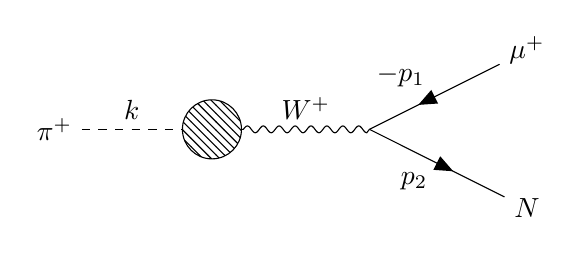
\begin{tikzpicture}
    \begin{feynman}
      \vertex [blob] (a) at (0, 0) {};
      \vertex (b) at (2, 0);
      \vertex (i1) at (-2, 0) {$\pi^+$};
      \vertex (f1) at (4, 1) {$\mu^+$};
      \vertex (f2) at (4, -1) {$N$};
      \diagram* {
      (i1) -- [scalar, edge label=$k$] (a),
      (a) -- [boson, edge label=$W^+$] (b),
      (f2) -- [anti fermion, edge label=$p_2$] (b) -- [anti fermion, edge label=$-p_1$] (f1),
      };
    \end{feynman}
  \end{tikzpicture}
\end{center}
由于 HNL 粒子通过混合角 $U_{\mu}$ 参加弱作用，$\pi^\pm$ 的衰变过程中，HNL 产生的衰变宽度与产生 $\nu_\mu$ 的宽度
只差一个混合角和运动学因子：
\begin{equation}
  \frac{\Gamma_{\pi \to \mu N}}{\Gamma_{\pi \to \mu \nu}} =
  |U_{\mu}|^2 \times \rho_\pi (m_N) \label{eq:pion_HNL_rho}
\end{equation}
其中
\begin{align}
   & \rho_\pi (m_N) = \frac{(m_\pi^2 (m_\mu^2 + m_N^2) - (m_\mu^2 - m_N^2)^2) \sqrt{\lambda(m_\pi^2, m_\mu^2, m_N^2)}}{m_\mu^2 (m_\pi^2 - m_\mu^2)^2} \label{eq:rho_pi} \\
   & \lambda(x, y, z) = x^2 + y^2 + z^2 - 2xy - 2yz - 2zx
\end{align}
此过程的运动学因子在 $m_N = \qtyrange{10}{30}{\mega\electronvolt}$ 的范围内从接近 1 下降到 0.7 左右，故主要的贡献在混合角，相空间抑制相比较而言不明显。

对于两体衰变，产物在质心系中的能量是固定的，能谱的分布来源于母粒子的能谱。HNL 在实验室系中的最大能量为
\begin{equation}
  \lambda_{max} = \frac{E_{N,max}}{E_\pi} = \frac{m_\pi^2 - m_\mu^2 + m_N^2 + \sqrt{\lambda(m_\pi^2, m_\mu^2, m_N^2)}}{2 m_\pi^2}
\end{equation}
当取 $m_N \to 0$ 时得到无质量中微子的情况 \cite{kelner2006energy}。在 $m_N = \qtyrange{10}{30}{\mega\electronvolt}$ 的范围内，这一比值从 0.42 下
降到 0.34 左右。而对中微子这一值为 $1 - m_\mu^2 / m_\pi^2 \approx 0.43$。有质量的 HNL 相比较中微子从 $\pi$ 介子中分得较少的能量。

这同时表明对于 $\pi$ 介子衰变产生 HNL 的过程，\parencite{kelner2006energy} 中对于中微子的表达式仍然适用，只需要替换上述比值即可。即对于已知的 $\pi$ 介子
谱，有
\begin{equation}
  Q_{N}(E_N) = \int_{\frac{E_N}{\lambda_{max}}}^{\infty} J(E_\pi) \frac{d E_\pi}{\lambda_{max} E_\pi} \label{eq:hnl_spec_from_pion}
\end{equation}

然而，由于 $\mu$ 子的质量相较于 HNL 较大，衰变过程中依然存在明显的螺旋性不对称。不同螺旋的 HNL 粒子会影响其衰变的角分布。在 $\pi$ 介子静止系
中，产生螺旋度 $-1$ 的 HNL 粒子与 $+1$ 的 HNL 粒子的衰变宽度由下式给出
\begin{equation}
  % \Gamma_{\pi \to N}^{(s)} \propto (m_\mu^2 + m_N^2) m_\pi^2 - (m_\mu^2 - m_N^2)^2 - s \cdot (m_\mu^2 - m_N^2) \sqrt{\lambda(m_\pi^2, m_\mu^2, m_N^2)}
  \frac{\Gamma_R}{\Gamma_L} = \frac{(m_\mu^2 + m_N^2) m_\pi^2 - (m_\mu^2 - m_N^2)^2 - (m_\mu^2 - m_N^2) \sqrt{\lambda(m_\pi^2, m_\mu^2, m_N^2)}}
  {(m_\mu^2 + m_N^2) m_\pi^2 - (m_\mu^2 - m_N^2)^2 + (m_\mu^2 - m_N^2) \sqrt{\lambda(m_\pi^2, m_\mu^2, m_N^2)}} \label{eq:hnl_hel_pion}
\end{equation}
其随 HNL 质量的变化在图 \ref{fig:spec_muon_HNL_pol} 中绘出。

然而，在高能标下，不同螺旋度的 HNL 粒子的衰变产物能谱并没有数量级上的差别，所以在针对天体的计算中，忽略产生的 HNL 的螺旋度是一可行的近似。

\subsection{$\mu$ 子衰变}
处理 $\mu$ 子衰变这样的三体衰变会更加繁琐，但事实上，与处理 $\pi \to \mu N$ 的过程一样，新过程只是标准模型产生中微子的衰变加上混合角和不可忽略的质量。
$\mu$ 子产生 HNL 粒子的衰变过程如下：
\begin{center}
  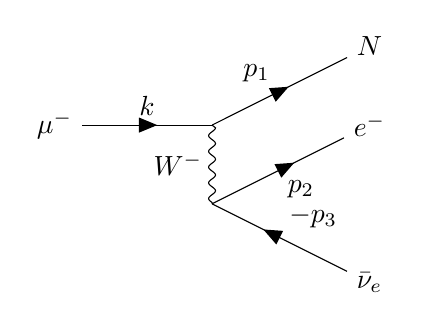
\begin{tikzpicture}
    \begin{feynman}
      \vertex (a) at (0, 0);
      \vertex (b) at (0, -1);
      \vertex (i1) at (-2, 0) {$\mu^-$};
      \vertex (f1) at (2, 1) {$N$};
      \vertex (f2) at (2, 0) {$e^-$};
      \vertex (f3) at (2, -2) {$\bar{\nu}_e$};
      
      \diagram* {
      (i1) -- [fermion, edge label=$k$] (a) -- [fermion, edge label=$p_1$] (f1),
      (b) -- [boson, edge label=$W^-$] (a),
      (f2) -- [anti fermion, edge label=$p_2$] (b) -- [anti fermion, edge label=$-p_3$] (f3),
      };
    \end{feynman}
  \end{tikzpicture}
\end{center}
其衰变宽度具有如下形式
\begin{equation}
  \frac{\Gamma_{\mu \to N}}{\Gamma_{\mu \to \nu}} = |U_{\mu}|^2 \times \rho_\mu(m_N)
\end{equation}
其中 HNL 的质量导致的运动学因子为
\begin{equation}
  \rho_\mu(m_N) = - r_N^8 + 8 r_N^6 - 24 r_N^4 \ln(r_N) - 8 r_N^2 + 1 \label{eq:rho_mu}
\end{equation}
其中 $r_N = m_N / m_\mu$。上式与 \cite{Bondarenko_2018} 中式（2.8）具有相同的形式，这是可以预见的，因为这个
衰变过程对于 $\mu$ 子和 $\tau$ 子是完全相似的。\ref{eq:rho_mu} 与 \ref{eq:rho_pi} 随 HNL 质量的变化同时在图
\ref{fig:spec_BR_HNL} 中绘出。可以看出在 HNL 质量较小时（< 10 MeV）
，由于质量带来的相空间抑制几乎可以忽略。而在接近相空间边缘处（30 MeV），在混合角外，质量将引入额外衰减，衰减
因子在 0.6 左右。

衰变产生的 HNL 能谱为：
\begin{equation}
  \frac{d\Gamma}{dE} = \frac{G_F^2 p^2 (3 m_\mu^2 E + 3 m_N^2 E - 4 m_\mu p - 6 m_N^2 m_\mu)}{12 \pi^3 E} \label{eq:mu_HNL_spec}
\end{equation}
在 $\mu$ 子静止系下，我们可以比较其产生的 HNL 和 $\nu_\mu$ 的能谱（图\ref{fig:spec_muon_HNL}），此图中 HNL 质量
$m_N = 20$ MeV。能谱对 $\nu_\mu$ 进行了归一化处理，并令 $|U_{\mu}|^2 = 1$。$\mu$ 子产
生 HNL 的情况下，产生的 HNL 能谱形状跟 $\nu_\mu$ 较为相似，除了由于 HNL 存在质量而导致的截断。这使得相
比于 $\nu_\mu$，HNL 的能谱略向高能集中一点，使得 HNL 倾向于携带更多能量。

如果对 $\mu$ 子的极化进行平均，在 $\mu$ 子静止系中，类似上文对 $\pi$ 介子的处理，可以得到产生左旋和右旋 HNL 粒子
的分支比。而由于 $\pi$ 介子衰变得到的 $\mu$ 子本身带有极化，这使得分析会极为复杂。对母粒子的螺旋度进平均
后的简化结果在图 \ref{fig:spec_muon_HNL_pol} 中绘出，相应的衰变宽度具有以下形式
\begin{equation}
  \begin{split}
    \Gamma_{\mu \to N}^{(s)} \propto \; & s \cdot (r_N^8-32 r_N^5+90 r_N^4-96 r_N^3+40 r_N^2-3) \\ 
                                        & -72 r_N^4 \, \ln{(r_N)} -3 r_N^8+24 r_N^6-24 r_N^2+3
  \end{split} \label{eq:mu_HNL_pol}
\end{equation}
其中 $s$ 是末态 HNL 的螺旋度。对于反 HNL 粒子，此过程是 CP 对称的。可以看出除非 HNL 的质量非常接近相空间边缘，HNL 
倾向以“正确的螺旋度”产生，取决于 HNL 的质量，$\pi$ 介子衰变中 2/3 以
上至几乎全部的 HNL 粒子是左旋的。与 $\pi$ 介子相比，$\mu$ 介子来源的 HNL 右旋和左旋之比随质量变大的上升趋势较弱，
这是因为三体衰变为角动量守恒创造了更灵活
的条件。

\begin{figure}[htbp]
  \centering
  \include{wxms/BR_compare_plot}
  \vspace{-1.5cm}
  \bicaption{不同 HNL 质量下 $\pi$ 介子与 $\mu$ 子衰变产生 HNL 的分支比。}{Branching ratios of HNL production from pion and muon decays as a function of HNL mass.}
  \label{fig:spec_BR_HNL}
\end{figure}

\begin{figure}[htbp]
  \centering
  \include{wxms/spectrum_plot.tex}
  \vspace{-1.5cm}
  \bicaption{在 $\mu$ 子静止系中，其衰变产生的有质量 HNL 和无质量 $\nu_\mu$ 的能谱比较。}{Comparison of the energy spectra of massive HNLs and massless $\nu_\mu$ produced in muon decays, evaluated in the muon rest frame.}
  % 。此图中 HNL 质量 $m_N = 20$ MeV。能谱对 $\nu_\mu$ 进行了归一化处理，并令 $|U_{\mu}|^2 = 1$。
  \label{fig:spec_muon_HNL}
\end{figure}


\begin{figure}[htbp]
  \centering
  \include{wxms/Muon_HNL_polarize.tex}
  \vspace{-1.5cm}
  \bicaption{母粒子静止系下，不同 HNL 质量下经由 $\pi$ 介子和 $\mu$ 子衰变产生右旋和左旋 HNL 的比。}{Ratio of right-handed to left-handed HNLs produced via pion and muon decays as a function of HNL mass, in the rest frame of the parent particle.}
  \label{fig:spec_muon_HNL_pol}
\end{figure}

\section{寿命与衰变}

\subsection{轻子衰变}
对于 HNL 粒子的衰变过程，其必须经由与 $\nu_\mu$ 的混合完成，考虑到我们研究的质量范围，其只能通过 $Z^0$ 通道衰变。
可能的通道有：
\begin{align*}
  N & \to \nu_\mu + e^- + e^+      \\
  N & \to \nu_\mu + \nu_l + \nu_l
\end{align*}
费曼图如下
\begin{center}
  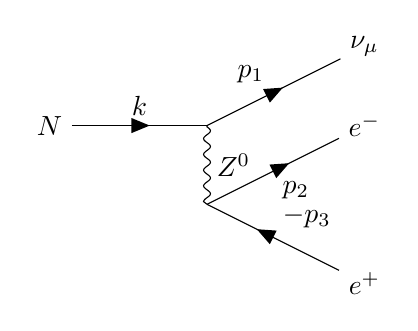
\begin{tikzpicture}
    \begin{feynman}
      \vertex (a) at (0, 0);
      \vertex (b) at (0, -1);
      \vertex (i1) at (-2, 0) {$N$};
      \vertex (f1) at (2, 1) {$\nu_\mu$};
      \vertex (f2) at (2, -0) {$e^-$};
      \vertex (f3) at (2, -2) {$e^+$};
      
      \diagram* {
      (i1) -- [fermion, edge label=$k$] (a) -- [fermion, edge label=$p_1$] (f1),
      (a) -- [boson, edge label=$Z^0$] (b),
      (f2) -- [anti fermion, edge label=$p_2$] (b) -- [anti fermion, edge label=$-p_3$] (f3),
      };
    \end{feynman}
  \end{tikzpicture}
  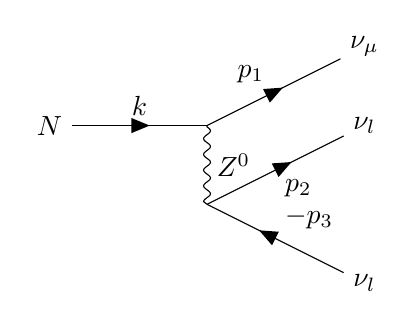
\begin{tikzpicture}
    \begin{feynman}
      \vertex (a) at (0, 0);
      \vertex (b) at (0, -1);
      \vertex (i1) at (-2, 0) {$N$};
      \vertex (f1) at (2, 1) {$\nu_\mu$};
      \vertex (f2) at (2, -0) {$\nu_l$};
      \vertex (f3) at (2, -2) {$\nu_l$};
      
      \diagram* {
      (i1) -- [fermion, edge label=$k$] (a) -- [fermion, edge label=$p_1$] (f1),
      (a) -- [boson, edge label=$Z^0$] (b),
      (f2) -- [anti fermion, edge label=$p_2$] (b) -- [anti fermion, edge label=$-p_3$] (f3),
      };
    \end{feynman}
  \end{tikzpicture}
\end{center}
这两个费曼图的计算在 \parencite{Bondarenko_2018} 中给出了如下结果
\begin{align}
  \Gamma_{N \to 3\nu}          & = \frac{G_F^2 m_N^5}{192 \pi^3} \times |U_\mu|^2 \label{eq:HNL_3nu_decay}               \\
  \Gamma_{N \to \nu e \bar{e}} & = \frac{G_F^2 m_N^5}{192 \pi^3} \times |U_\mu|^2 \times C_1^e \label{eq:HNL_nuee_decay}
\end{align}
上面两式已忽略电子质量，并且在产物全部为中微子的宽度中计入了所有不同味的情况，其中
\begin{equation}
  C_1^e = \frac{1}{4}\left(1 - 4 \sin^2 \theta_W + 8 \sin^4 \theta_W\right)
\end{equation}
在这种情况下产生电子的分支比约为
\begin{equation}
  BR_{N \to \nu e \bar{e}} = \frac{C_1^e}{1 + C_1^e} \approx 0.11
\end{equation}
这意味着 HNL 的电子衰变通道相比全不可见的中微子衰变（能量损失）受到抑制，会使产生的 HNL 的能谱
再衰减一个量级，这是因为中性弱作用对带电轻子和中微子的不同偶合。如果考虑电子的质量，低质量 HNL
将受到额外的相空间衰减，算出的分支比会更低。

\begin{figure}[htbp]
  \centering
  \include{wxms/HNL_lifetime.tex}
  \vspace{-1.0cm}
  \bicaption{仅考虑式 \ref{eq:HNL_3nu_decay} 与式 \ref{eq:HNL_nuee_decay} 通道时 HNL 粒子在不同质量下的寿命。}{HNL lifetime as a function of mass, considering only the decay channels in Eqs. \ref{eq:HNL_3nu_decay} and \ref{eq:HNL_nuee_decay}.}
  \label{fig:HNL_lifetime}
\end{figure}

根据上述衰变通道和宽度，计算出的 HNL 寿命如图 \ref{fig:HNL_lifetime} 所示。在 $\frac{m_e}{m_N} \ll 1$ 的情况
下，HNL 寿命与质量的 5 次方成反比，在对数坐标下是一条直线。考虑到混合角最大也不超过 $10^{-3}$，
我们所考虑的 HNL 的寿命至少在秒量级，寿命较长。

由于产生的 HNL 粒子具有螺旋度不对称，计算产物能谱时需要考虑 HNL 粒子的初态极化，这与 \cite{kelner2006energy} 中
对带有极化的 $\mu$ 子进行的讨论类似，不过由于弱中性流含有混合，形式会更为复杂。
考虑初态自旋的 HNL 静止系下
产生电子（或正电子）的能量与角分布函数为
\begin{equation}
  \begin{split}
    g_e^{(1)}(x, \cos{\theta}) = & \frac{8}{C_1^e} \cdot x^2 \cdot \{ [(4 - 16 s_W^2 + 64 s_W^4) x - (1 - 4 s_W^2 + 28 s_W^4)] \cos{\theta} \\
                                 & - (4 - 16 s_W^2 + 64 s_W^4) x + (3 - 12 s_W^2 + 36 s_W^4) \} \label{eq:g_e_p2}
  \end{split}
\end{equation}
\begin{equation}
  \begin{split}
    g_e^{(2)}(x, \cos{\theta}) = & \frac{16}{C_1^e} \cdot x^2 \cdot \{ [(6 - 24 s_W^2 + 32 s_W^4) x - (3 - 12 s_W^2 + 14 s_W^4)] \cos{\theta} \\
                                 & - (6 - 24 s_W^2 + 32 s_W^4) x + (3 - 12 s_W^2 + 18 s_W^4) \} \label{eq:g_e_p3}
  \end{split}
\end{equation}
其中 $x = E_e / m_N$ ， $s_W = \sin{\theta_W}$， $\theta$ 是出射电子与 HNL 自旋方向的夹角。式（\ref{eq:g_e_p2}）和式（\ref{eq:g_e_p3}）分别代表上面费曼图中
$p_2$ 和 $p_3$ 动量对应产生的粒子。

假设在实验室系中 HNL 具有确定的螺旋度，则实验室系中得到的电子谱线可以卷积得到为
\begin{equation}
  Q_e^{(Lab)}(E) = \int_{E}^{+\infty} d E_N \, Q_N^{(Lab)}(E_N) \int_{\frac{E}{2 E_N}}^{\frac{1}{2}}  \frac{d x}{x E_N} \, \sum_{i=1,2} g_e^{(i)}(x, s (\frac{E}{x E_N} - 1))
\end{equation}
其中 $s$ 为螺旋度，且 $+1,-1$ 分别表示 HNL 粒子为右旋与左旋。代入式 \ref{eq:g_e_p2} 和式 \ref{eq:g_e_p3} 后积分可以得到
\begin{equation}
  \int_{E}^{+\infty} \frac{d E_N}{E_N} \, Q_N^{(Lab)}(E_N) [16 y^3 - 27 y^2 + 11 -  s \cdot (32 y^3 - 63 y^2 + 36 y - 5) ]
\end{equation}
其中 $y=E/E_N$，在此式中弱混合角的参数被抵消了。对于不考虑 HNL 螺旋度的情况，取 $s=0$ 即可达到对螺旋度平均的效果。

\subsection{辐射衰变}
考虑圈图的情况下，HNL 可以通过味道改变中性流发生辐射衰变，直接产生 $\gamma$ 射线。典型的费曼图如下（还有另一个经由 $\mu$ 子发射光子的图）：
\begin{center}
  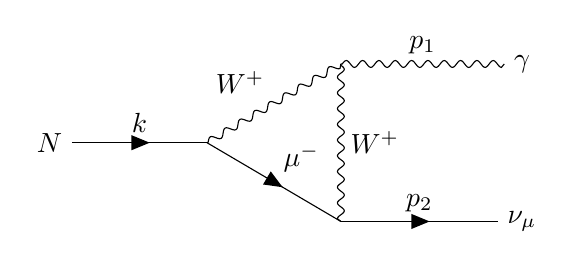
\begin{tikzpicture}
    \begin{feynman}
      \vertex (a) at (0, 0);
      \vertex (b) at (1.7, 1);
      \vertex (c) at (1.7, -1);
      \vertex (i1) at (-2, 0) {$N$};
      \vertex (f1) at (4, 1) {$\gamma$};
      \vertex (f2) at (4, -1) {$\nu_\mu$};
      \diagram* {
      (i1) -- [fermion, edge label=$k$] (a) -- [fermion, edge label=$\mu^-$] (c) -- [fermion, edge label=$p_2$] (f2),
      (a) -- [boson, edge label=$W^+$] (b) -- [boson, edge label=$W^+$] (c),
      (b) -- [boson, edge label=$p_1$] (f1),
      };
    \end{feynman}
  \end{tikzpicture}
\end{center}
然而，虽然我们在本文章中只考虑 HNL 与 $\nu_\mu$ 的混合，在典型的 ISS 模型中，HNL 会与所有味的中微子混合。这意味着此过程
会受到 GIM 机制的抑制，难以主导衰变过程。如果我们考虑其它机制产生的辐射衰变，
情况会有所不同。
引入一个不可重整的有效场论算符有 \cite{Magill_2018}
\begin{equation}
  \mathcal{L}_{int} = \frac{d}{2} \bar{\nu}_L \sigma_{\mu \nu} F^{\mu \nu} N + h.c. \label{eq:int_mag_nu}
\end{equation}
这是一个偶极相互作用。如果 HNL 粒子通过 ISS 混合产生，而通过偶极辐射衰变，如果偶极耦合常数合适，其寿命可以在秒至亚秒量级
，并保证辐射衰变相比其它 ISS 混合衰变占据主导，使 HNL 的衰变过程与混合角 $|U_\mu|^2$ 近似地解耦。偶极辐射衰变的
衰变宽度为 \cite{Magill_2018}
\begin{equation}
  \Gamma_{N \to \nu \gamma} = \frac{|d|^2 m_N^3}{8 \pi}
\end{equation}
其对应的费曼图如下
\begin{center}
  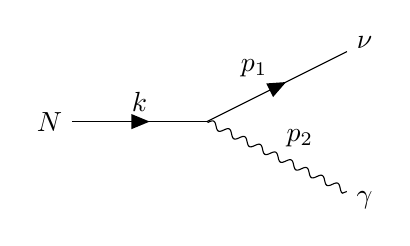
\begin{tikzpicture}
    \begin{feynman}
      \vertex (a) at (0, 0);
      \vertex (i1) at (-2, 0) {$N$};
      \vertex (f1) at (2, 1) {$\nu$};
      \vertex (f2) at (2, -1) {$\gamma$};
      \diagram* {
      (a) -- [boson, edge label=$p_2$] (f2),
      (i1) -- [fermion, edge label=$k$] (a) -- [fermion, edge label=$p_1$] (f1),
      };
    \end{feynman}
  \end{tikzpicture}
\end{center}
而考虑初态 HNL 极化的情况下，在 HNL 静止系中，产生光子的角分布为
\begin{equation}
  % \frac{d \Gamma}{d \Omega} = \frac{|d|^2}{16 \pi^2} m_N^3 (1 + \cos{\theta_{s}})
  \frac{d \Gamma}{d \Omega} \propto 1 + \cos{\theta_{s}} \label{eq:HNL_gamma_spec_d}
\end{equation}
对上式进行洛伦兹 Boost 后得到 HNL 衰变光谱，
左旋和右旋 HNL，其产生的 $\gamma$ 光子谱有会有所区别
\begin{equation}
  Q_\gamma^{(s)} (E) = \frac{1}{\beta_N \gamma_N m_N} \left[ \left( 1 - \frac{s}{\beta_N}\right) + \frac{2 s E}{\beta_N \gamma_N m_N} \right]
\end{equation}
其中 
\begin{align*}
   & \frac{m_N}{2} \gamma_N (1 - \beta_N) < E < \frac{m_N}{2} \gamma_N (1 + \beta_N)
   & s = +1,-1
\end{align*}
$\gamma_N$ 是到 HNL 静止系的洛伦兹 Boost 因子。
这两个公式可以用于任何 HNL 处于确定螺旋度的参考系中。对于 $\pi$ 介子产生的 HNL，上述两式的权重
由 \ref{eq:hnl_hel_pion} 给出，这种情况下参考系为 $\pi$ 介子静止系。上面两式的差别可以解读为
由于中微子必须是左旋的，所以左旋 HNL 要发射光子必须沿向反方向发射以保证角动量守恒，这使得在
洛伦兹 Boost 后光子能量降低，而右旋 HNL 则反之。

如果只考虑 $\pi$ 介子直接产生的 HNL，在实验室系下的 $\gamma$ 谱线通过卷积可以得到：
\begin{equation}
  Q_{\gamma}^{(Lab)} (E) = \int_{E_{\gamma min}^{(\pi)}}^{E_{\gamma max}^{(\pi)}} d E_\gamma^{(\pi)} \; Q_\gamma^{(\pi)}(E_\gamma^{(\pi)}) \int_{\frac{m_\pi E}{2 E_\gamma^{(\pi)}}}
  ^{+\infty} J_\pi (E_\pi) \; \frac{d E_\pi}{2 \gamma_\pi(E_\pi) \; E_\gamma^{(\pi)}}
\end{equation}
与式 \ref{eq:hnl_spec_from_pion} 类似，这里假设 $\pi$ 介子能量极高的相对论情况。

另一方面，考虑近似情况，若认为所有的 HNL 都是左旋的，则 $\gamma$ 谱线可以直接由 HNL 谱得到（取相对论极限）
\begin{equation}
  % Q_\gamma^{(Lab)} (E) = \int_{E}^{+\infty} Q_N(E_N) \frac{d E_N}{E_N} \label{eq:pure_L_N_gamma}
  Q_\gamma^{(Lab)} (E) = \int_{E}^{+\infty}d E_N \, Q_N(E_N) \, \frac{2 (E_N - E)}{E_N^2} \label{eq:pure_L_N_gamma}
\end{equation}
上式其实是式 \ref{eq:hnl_spec_from_pion} 的简化版本，因为此处的衰变产物的质量在计算过程中被忽略，所以 $\lambda$ 因子被简化了。

上述关于HNL的产生与衰变机制不仅在粒子物理唯象学中具有重要意义，更为解释极端天体环境中的多信使观测结果提供了关键
的物理图像。
在 AGN 的核心区域，强烈的质子相互作用提供了丰富的 $\pi$ 介子与 $\mu$ 子，进而大量产生HNL。
由于 HNL 具有较弱的相互作用和较长的寿命（如2.3节所述），它们能够像中微子一样穿透对高能光子不透明的 AGN
冕区。当这些HNL在逃逸至视界外且稀薄的区域后发生衰变（无论是产生电子再发生逆康普顿散射，还是直接发生辐射
衰变），就能转化为可逃逸并被地球探测器捕捉到的高能 $\gamma$ 光子。下一章，我们将把这一理论模型具体应用于NGC 1068的
天文观测中，探讨其在实际多信使信号中的应用潜力。

\chapter{实验观测与模型应用}

\section{NGC 1068 的多信使观测现状与物理背景}

NGC 1068 距离地球约 14.4 Mpc，是研究最为充分的明亮塞弗特（Seyfert II）活动星系核之一。近期，IceCube中微子天文台
在TeV能量范围内确认了来自该源的高能中微子辐射。根据标准的天体物理模型，AGN环境中的质子-质子（$pp$）和质子-光子
（$p\gamma$）相互作用在产生高能中微子的同时，不可避免地会伴生相同量级的高能$\gamma$射线。

然而，多波段的电磁观测表明，NGC 1068在GeV至TeV波段的$\gamma$射线通量远低于由中微子通量所预期的理论值。
这种“中微子明亮但$\gamma$射线暗淡”的现象表明，NGC 1068的源区（如黑洞吸积盘附近的冕区）存在极高的光深，
对高能$\gamma$光子是极其不透明的（即被致密物质或辐射场遮蔽和吸收）\cite{murase2020hidden}。而如果存在
某种弱相互作用的粒子，如 HNL，在 AGN 核中的产生，其就有可能将能量带出不透明的区域，如果同时存在可见的衰变通道，就
可能产生可观测的信号。这也为解释现有的级联模型中的虽然解释了远低于中微子的 $\gamma$ 通量，但实际观测却
仍存在一定通量的矛盾提供了新思路。

\section{通量估算}

根据 \parencite{icecube2022evidence} 的观测分析，来自 NGC 1068 的中微子通量可以简化地描述为
\begin{equation}
  \Phi_{\nu_\mu + \bar{\nu}_\mu} = \Phi_0 \cdot (\frac{E_\nu}{E_0})^{-\gamma} \label{eq:icecube_nuspec}
\end{equation}
此表达式是 IceCube 观测到的中微子谱在 1.5TeV 至 15TeV 范围内的通量。\parencite{murase2020hidden} 中理论分析建立了完整的 $\nu$ 能谱。
AGN 中的中微子产生主要由 $pp$ 过程和 $p\gamma$ 过程主导 \cite{murase2020hidden}。而 $pp$ 过程和 $p\gamma$ 过程产生的中微子
都来自于其直接产物 $\pi$ 介子的衰变，并在同一过程中产生相应的 $\gamma$ 射线。

根据 \parencite{kelner2006energy} 中的结论，中微子的能谱由 $\pi$ 介子的注入能谱决定，
\begin{align}
  Q_{\nu_\mu}(E_{\nu_\mu}) & = 2 \int_{0}^{1} (f_{\nu_\mu^{(1)}}(x) + f_{\nu_\mu^{(2)}}(x)) \; J_\pi\left(\frac{E_{\nu_\mu}}{x}\right) \frac{dx}{x} \\
  Q_{\nu_e}(E_{\nu_e})     & = 2 \int_{0}^{1} f_{\nu_e}(x) \; J_\pi\left(\frac{E_{\nu_e}}{x}\right) \frac{dx}{x}
\end{align}
其中 $f_{i^{(j)}}$ 是不同的核函数。利用上式，假设产生的 $\pi$ 介子与 $\nu$ 共享相同的谱形状，可以拟合出 NGC 1068 中产生
的 $\pi$ 介子谱。

考虑到 $m_N \leq 30 \text{MeV}$ 的情况下 HNL 质量对过程没有巨大影响，直接利用 $\nu_\mu$ 谱线结合 $|U_\mu|^2$
进行衰减是一个良好的近似。 
若假设 HNL 产生的运动学与 $\nu_\mu$ 完全相同，又考虑到中微子味振荡的作用，HNL 的能谱为
\begin{equation}
  \Phi_N (E) = |U_\mu|^2 \cdot (\rho_\pi + \rho_\mu) \cdot \Phi_{\nu_\mu + \bar{\nu}_\mu} (E) \label{eq:approx_spec}
\end{equation}
上式是一个粗略的近似，除了忽略运动学不同之外，直接对两种不同过程的分支比取平均存在一定问题，因为 $\pi$ 介子和 $\mu$ 子并不完全相同
地贡献不同能量下的 HNL 通量。但如图 \ref{fig:spec_BR_HNL} 所示，不存在数量级上的差别。使用上式近似的好处是可以直接建立由中微子到
HNL 的估算关系，而不用依赖于具体的 AGN 模型对 $\pi$ 介子谱线的估算。
在这种情况下，如果假设所有的 HNL 粒子都经由式 \ref{eq:int_mag_nu} 所描述的相互作用衰变，套用式 \ref{eq:pure_L_N_gamma} 可以算得经
HNL 衰变的 $\gamma$ 能谱（图 \ref{fig:gamma_spec_U_2}）。图中红色实线为估算结果，其它是来自文献 \cite{icecube2022evidence}
的理论值和观测结果。参数取值为
$|U_\mu|^2 = 10^{-2}$，且 $m_N \ll m_\mu, m_\pi$，假设 HNL 产生的动力学与 $\nu_\mu$ 完全相同，且全部为左旋。
可以看出 HNL 衰变的 $\gamma$ 谱线由于
存在额外的一级衰变过程，有一定的展宽。
配合现存的 $\gamma$ 射线观测结果，可以用于推断 $|U_\mu|^2$ 的上限，
图 \ref{fig:U_UL_approx} 给出了特定近似和假设下的限制。此限制并非严格的单独 ISS 机制混合角
限制，因为它假设 HNL 具有辐射衰变主导的这一特性。如果 HNL 的辐射衰变占比很小，那么如下面将讨论的，几乎无法通过
NGC 1068 对 HNL 混合角 $|U_\mu|$ 进行限制。

如果 HNL 不存在直接的辐射衰变通道，或者相比 ISS 机制的衰变不占主导，那么主要的可观测衰变将是电子衰变。高能电子再经过对星际空间中宇宙
微波背景的逆康普顿散射，产生 $\gamma$ 射线。同样地，可以忽略产生的 HNL 的极化，直接对两极化平均。对于产生电子如何转化为 $\gamma$ 射线，
可以使用简单的 $\delta$ 假设，即某一能量的 $\gamma$ 光子完全来自于相应能量的电子。能量关系可以表示为 \cite{RevModPhys.42.237}
\begin{equation}
  E_\gamma \approx \frac{4}{3} \left( \frac{E_e}{m_e} \right)^2 \epsilon_0
\end{equation}
电子谱经由逆康普顿散射得到的光子谱可以由一个简单的缩放关系得到
\begin{equation}
  Q_\gamma(E_\gamma) = \frac{E_e}{2 E_\gamma} Q_e(E_e) 
\end{equation}
经由此过程的 $\gamma$谱线估算在图 \ref{fig:U_UL_approx} 中绘出。参数取值为
$|U_\mu|^2 = 10^{-1}$，且 $m_N \ll m_\mu, m_\pi$，假设 HNL 产生的动力学与 $\nu_\mu$ 完全相同，且全部为左旋。此种情况下产生电子的衰变本身已受到
抑制，再经由与微波背景的逆康普顿散射之后，产生的 $\gamma$ 射线通量比当前探测低数个量级，几乎不存在探测到的可能，也无法对参数空间给出有意义的限制。

\begin{figure}[htbp]
  \centering
  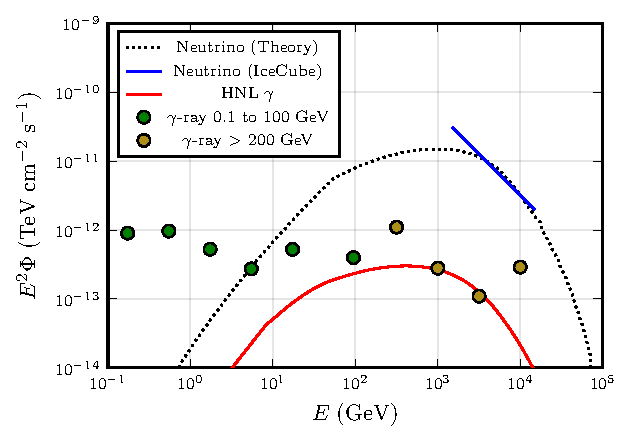
\includegraphics[width=0.7\textwidth]{julia_plots/u1.5_gamma.pdf}
  \bicaption{NGC 1068 经 HNL 衰变的 $\gamma$ 射线估算结果（基于辐射衰变主导假设）。}{Estimated $\gamma$-ray fluxes from HNL decays in NGC 1068 (under the assumption of dominant radiative decay).}
  \label{fig:gamma_spec_U_2}
\end{figure}

\begin{figure}[htbp]
  \centering
  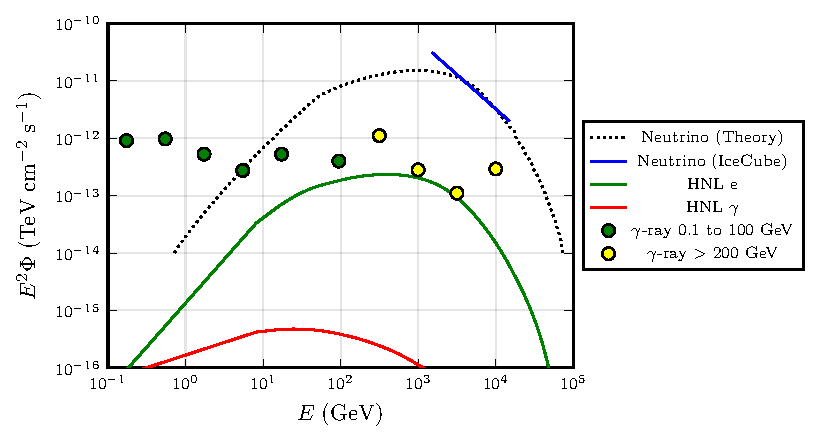
\includegraphics[width=0.7\textwidth]{julia_plots/u_e_gamma.pdf}
  \bicaption{NGC 1068 经 HNL 衰变的 $\gamma$ 射线估算结果（仅考虑 ISS 机制轻子衰变）。}{Estimated $\gamma$-ray fluxes from HNL decays in NGC 1068 (considering only leptonic decays within the ISS mechanism).}
  \label{fig:gamma_spec_U_1_e}
\end{figure}

\begin{figure}[htbp]
  \centering
  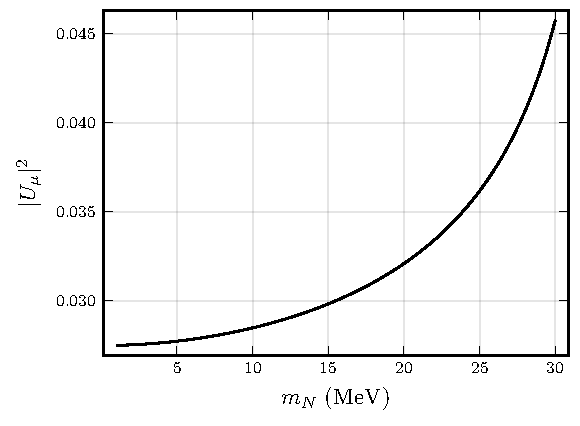
\includegraphics[width=0.4\textwidth]{julia_plots/U_UL.pdf}
  \bicaption{$|U_\mu|^2$ 的上限限制}{Upper limits on $|U_\mu|^2$.}
  \label{fig:U_UL_approx}
\end{figure}

\chapter{结论与展望}

随着IceCube等大型探测器积累了大量数据，多信使天文学正成为探索极端天体物理和超越标准模型（BSM）新物理的重要交叉领域。
本文以AGN NGC 1068中微子与 $\gamma$ 射线的通量异常为切入点，系统研究了重中性轻子（HNL）在这一天体物理环境中的产生与
输运机制。本研究不仅为解释 NGC 1068 的高能 $\gamma$ 射线提供了一种基于BSM的替代方案，也展示了利用大尺度天文现象
限制微观粒子参数空间的独特优势。

本文针对质量在 30 MeV 以下的HNL粒子进行了详细的唯象学计算与唯象模型应用，取得以下主要成果：
\begin{enumerate}
  \item 推导了 AGN 高能背景下，HNL 经由 $\pi$ 介子和 $\mu$ 子衰变的产生分支比及能谱特征，发现 HNL 由于质量导致的截断效应使其倾向于携带更高的能量；
  \item 评估了 HNL 的轻子衰变通道。在仅考虑 ISS 机制的情况下，由于电子衰变受抑制及转换通量的损失，产生的 $\gamma$ 射线信号极其
        微弱，在当前及未来的观测精度下均难以被探测；
  \item 若引入额外的有效算符使得 HNL 偶极辐射衰变占主导，HNL 在逃逸出AGN冕区后可以直接转化为 $\gamma$ 光子。利用这一机制计算所得的 $\gamma$ 射线
        谱能够在一定程度上匹配观测结果，并以此推断给出了 HNL 混合角 $|U_\mu|^2$ 在特定质量范围内的上限限制。
\end{enumerate}

尽管本文证实了HNL模型在解释NGC 1068多信使信号方面的潜力，但在理论计算中仍存在许多近似与不足。例如，计算中忽略了由于弱相互作用宇称不守恒
导致产生的HNL螺旋度极化效应；模型假设了HNL完全在冕区外且全部在地球视界内衰变，这需要结合更精确的 AGN 模型进行三维蒙特卡洛模拟。
此外，占主导的纯偶极辐射衰变的参数空间已受到超新星观测的部分限制。

展望未来，随着新一代中微子观测站（如KM3NeT/ARCA）以及更高灵敏度的 $\gamma$ 射线天文台（如CTA）的建成并投入运行，更多像 NGC 1068 这样的点源将
被精细测量。结合更严谨的宇宙线输运模拟与粒子物理计算，我们有望对HNL的参数空间进行更严格的压缩，甚至在极端的宇宙实验室中真正捕捉到来自HNL衰变
的明确信号。


\backmatter


% 打印参考文献
\PrintReference

% 附录
\begin{appendix}
  \setcounter{equation}{0}
  \renewcommand{\theequation}{A.\arabic{equation}}
  \renewcommand{\labelenumi}{(\arabic{enumi})}
  \begin{enumerate}
    \item $\pi$ 介子衰变成 HNL 粒子，相应费曼图见 2.2.1，振幅为
          \begin{equation}
            \mathcal{M} = \frac{f_\pi g_w^2}{8 M_W^2} k^\mu [\bar{u}(p_2) \gamma_\mu (1 - \gamma^5) v(p_1)]
          \end{equation}
          根据求解费曼图的一般过程，即重新排列旋量后使用求迹，即可求出相应的衰变宽度。而如果需要考虑末态 HNL 粒子的
          自旋，则在计算振幅模平方时应使用如下的关系
          \begin{equation}
            u(p_2) \bar{u}(p_2) = (\slashed{p}_2 + m_N) \frac{1 + \slashed{s}}{2}
          \end{equation}
          其中 $s^\mu$ 是 HNL 粒子的自旋四矢量。在静止系下，自旋沿 $z$ 轴正/负方向的自旋四矢量为
          \begin{equation}
            s_{rest}^\mu = (0, 0, 0, s) \label{eq:s_rest}
          \end{equation}
          其中 $s=\pm 1$ 而在 HNL 非静止的系中，则对其做一次洛伦兹 Boost。在 $\pi$ 介子衰变的过程中，我们取 $\pi$
          介子静止系，并令 $p_2$ 沿 $z$ 轴正方向，有
          \begin{equation}
            s^\mu = \Lambda^\mu_\nu s_{rest}^\nu = \left(\frac{|p_2|}{m_N} s, 0, 0, \frac{\sqrt{|p_2|^2 + m_N^2}}{m_N} s\right)
          \end{equation}
          而得出的振幅模平方为
          \begin{equation}
            \langle |\mathcal{M}| \rangle^2 = \frac{1}{16} \left[ f_\pi^2 \left( \frac{g_w}{M_W} \right)^2 \right]^2 [ 2 (k \cdot p_1) (k \cdot p_2) - k^2 (p_1 \cdot p_2) + 2 m_N (k \cdot p_1) (k \cdot s) - m_N k^2 (p_1 \cdot s) ]
          \end{equation}
          对于两体衰变，所有四动量都有确定值，代入即可得到式 \ref{eq:hnl_hel_pion}。如果对 $s=\pm 1$ 两种情况求和，
          则可以得到式 \ref{eq:pion_HNL_rho}。
          
    \item $\mu$ 子衰变成为 HNL，相应费曼图见 2.2.2
          \begin{equation}
            \mathcal{M} = 2\sqrt{2} G_F [\bar{u}(p_1) \gamma_\mu P_L u(k)] \cdot [\bar{u}(p_2) \gamma^\mu P_L v(p_3) ]
          \end{equation}
          同样保留 HNL 粒子的自旋，振幅模平方的形式则较简洁，有
          \begin{equation}
            \langle |\mathcal{M}| \rangle^2 = 32 G_F [(k \cdot p_3)(p_1 \cdot p_2) - m_N (k \cdot p_3) (p_2 \cdot s)]
          \end{equation}
          消去 $p_2$ 并重新整理，可以得到
          \begin{equation}
            \begin{split}
              \langle |\mathcal{M}| \rangle^2 & = 32 G_F^2 m_\mu |\overrightarrow{p}_3| [ \frac{1}{2}(m_\mu^2 - m_N^2)  - |\overrightarrow{p}_3| m_\mu                                  \\
                                              & - s \left(m_\mu |\overrightarrow{p}_1| - |\overrightarrow{p}_3| |\overrightarrow{p}_1| + |\overrightarrow{p}_3| \cos{θ_3} E_1\right) ]
            \end{split}
          \end{equation}
          其中 $E_1=\sqrt{|\overrightarrow{p}_1|^2 + m_N^2}$。积分以得到衰变宽度有
          \begin{equation}
            d \Gamma = \frac{1}{16(2\pi)^4 m_\mu} \frac{d^3 \overrightarrow{p}_1}
            {|\overrightarrow{p}_1| \cdot E_1} d |\overrightarrow{p}_3| \int_{u_-}^{u_+} \langle |\mathcal{M}| \rangle^2 \delta(m_\mu - E_1 - |\overrightarrow{p}_3| - u) \, d u
          \end{equation}
          其中 $u^2 \equiv |\overrightarrow{p}_1 + \overrightarrow{p}_3|^2$。完成对 $u$ 的积分有
          \begin{equation}
            \Gamma = \frac{1}{(4\pi)^4 m_\mu} \int \frac{d^3 \overrightarrow{p}_1}{|\overrightarrow{p}_1| \cdot E_1} \int_{|\overrightarrow{p}_3|_{-}}^{|\overrightarrow{p}_3|_{+}}
            d |\overrightarrow{p}_3| \langle |\mathcal{M}| \rangle^2
          \end{equation}
          由于 $\delta$ 函数的选择性，以及为保证 $\delta$ 函数不为 0，需要
          \begin{align}
            \cos{\theta_3}               & = \frac{2 |\overrightarrow{p}_3| (E_1 - m_\mu) -2 m_\mu E_1 + m_\mu^2 + m_N^2}{2 |\overrightarrow{p}_1| |\overrightarrow{p}_3|} \\
            |\overrightarrow{p}_3|_{\pm} & = \frac{1}{2}(m_\mu \pm |\overrightarrow{p}_1| - E_1)                                                                           \\
          \end{align}
          且
          \begin{equation}
            0 < |\overrightarrow{p}_1| < \frac{m_\mu^2-m_N^2}{2 m_\mu}
          \end{equation}
          完成积分，并按照对应极化态代入 $s$ 即可得到式 \ref{eq:rho_mu}、\ref{eq:mu_HNL_spec}、\ref{eq:mu_HNL_pol}。
          
    \item HNL 粒子衰变的过程，取 HNL 静止系，则自旋四矢量保持 $(0,0,0,1)$，而只需在进行洛伦兹 Boost 时注意对应的角度的正反即可。
          先考虑 HNL 的辐射衰变，根据 \ref{eq:int_mag_nu} 给出的作用量，相应的费曼顶角为
          \begin{equation}
            i \, 2 \, d \, \sigma^{\alpha\beta} q_\beta P_R
          \end{equation}
          费曼图见 2.3.2 对应的衰变振幅为
          \begin{equation}
            \mathcal{M} = 2i \, d [\bar{u}(p_1) \sigma^{\alpha\beta} p_{2\beta} P_R u(k)] \epsilon_\alpha(p_2)
          \end{equation}
          而振幅模方则为
          \begin{equation}
            \langle |\mathcal{M}| \rangle^2 = 4 |d|^2 m_N^3 [m_N + 2 (p_2 \cdot s)] 
          \end{equation}
          代入 $p_2 \cdot s = \frac{m_N}{2} \cos{\theta_s}$ 即可得到式 \ref{eq:HNL_gamma_spec_d}。
          
          本文研究的 HNL 衰变成为电子的过程是一弱中性过程，因而顶角会带有弱混合角，费曼图见 2.3.1
          \begin{equation}
            \mathcal{M} = \frac{G_F}{\sqrt{2}} [\bar{u}(p_1) \gamma^\mu P_L u(k)] \cdot [ \bar{u}(p_2) (2 s_W^2 - P_L) v(p_3)]
          \end{equation}
          保留 HNL 粒子的自旋会使振幅模平方变得极为复杂
          \begin{equation}
            \begin{split}
              \langle |\mathcal{M}| \rangle^2 = \frac{G_F^2}{2} \{ & - 8 m_N^2 |\overrightarrow{p}_3|^2 + 4 m_N^3 |\overrightarrow{p}_3| + 32  s_W^2 m_N^2 |\overrightarrow{p}_3|^2 - 16  s_W^2 m_N^3 |\overrightarrow{p}_3|                                                                                                     \\
                                                                   & - 32  s_W^4 m_N^2 |\overrightarrow{p}_3|^2 - 32  s_W^4 m_N^2  |\overrightarrow{p}_2|^2 + 16  s_W^4 m_N^3 |\overrightarrow{p}_3|                                                                                                                             \\
                                                                   & + 16  s_W^4 m_N^3  |\overrightarrow{p}_2| + 32  |\overrightarrow{p}_2| \cos{\theta_2}  s_W^4 m_N^2  |\overrightarrow{p}_2| - 16  |\overrightarrow{p}_2| \cos{\theta_2}  s_W^4 m_N^3 + 8  |\overrightarrow{p}_3| \cos{\theta_3} m_N^2 |\overrightarrow{p}_3| \\
                                                                   & - 4  |\overrightarrow{p}_3| \cos{\theta_3} m_N^3 - 32  |\overrightarrow{p}_3| \cos{\theta_3}  s_W^2 m_N^2 |\overrightarrow{p}_3| + 16  |\overrightarrow{p}_3| \cos{\theta_3}  s_W^2 m_N^3                                                                   \\
                                                                   & + 32  |\overrightarrow{p}_3| \cos{\theta_3}  s_W^4 m_N^2 |\overrightarrow{p}_3| - 16  |\overrightarrow{p}_3| \cos{\theta_3}  s_W^4 m_N^3 \}
            \end{split}
          \end{equation}
          要计算末态电子的能谱，以 $p_3$ 对应的电子为例，则应先完成对 $\theta_2$ 的积分。设 $\overrightarrow{p}_2$ 与 $\overrightarrow{p}_3$ 间的夹角为 $\alpha$，进行换元 $u^2 \equiv |\overrightarrow{p}_2 + \overrightarrow{p}_3|^2$，可以完成对 $\alpha$ 的积分，
          而 $\cos{\theta_2} = \cos{\alpha} \cos{\theta_3} + \sin{\alpha} \sin{\theta_3} \cos{\varphi}$。
          从 $\delta(m_N - |\overrightarrow{p}_2 + \overrightarrow{p}_3| - |\overrightarrow{p}_2| - |\overrightarrow{p}_3|)$ 中可以求解出
          \begin{equation}
            \cos{\alpha} = \frac{m_N^2}{2|\overrightarrow{p}_2||\overrightarrow{p}_3|}-\frac{m_N}{|\overrightarrow{p}_3|}-\frac{m_N}{|\overrightarrow{p}_2|}+1
          \end{equation}
          为了保证 $\delta$ 函数不为 0，需要 $ \frac{m_N}{2} - |\overrightarrow{p}_3| < |\overrightarrow{p}_2| < \frac{m_N}{2}$。至此可以完成对 $|\overrightarrow{p}_2|$ 的积分。
          
          同时由于 $0 < \varphi < 2 \pi$，$\varphi$ 也可以容易地积分掉，积分中将只剩下 $|\overrightarrow{p}_3|$ 与 $\cos{\theta_3}$，可以得出
          \begin{equation}
            \begin{split}
              \frac{d \Gamma}{d |\overrightarrow{p}_3| \, d\cos{\theta_3}} = & \frac{4 G_F \pi m_N^2}{3} |\overrightarrow{p}_3|^2                                                                                \\
                                                                             & \cdot (32 |\overrightarrow{p}_3| s_W^4 \cos{\theta_3}-14 m_N s_W^4 \cos{\theta_3} -24 |\overrightarrow{p}_3| s_W^2 \cos{\theta_3} \\
                                                                             & +12 m_N s_W^2 \cos{\theta_3} +6 |\overrightarrow{p}_3| \cos{\theta_3}-3 m_N \cos{\theta_3}-32 |\overrightarrow{p}_3| s_W^4        \\
                                                                             & +18 m_N s_W^4+24 |\overrightarrow{p}_3| s_W^2-12 m_N s_W^2-6 |\overrightarrow{p}_3|+3 m_N)
            \end{split}
          \end{equation}
          用同样的方式处理 $p_2$ 所对应的粒子并相加，就可以得到考虑 HNL 自旋的 HNL 衰变的电子/正电子产物能谱和角分布，即式 \ref{eq:g_e_p2} 和 \ref{eq:g_e_p3}。
          
  \end{enumerate}
  
\end{appendix}

% 致谢
\begin{acknowledgement}
  首先衷心感谢阮建红教授在课题选择、研究和论文撰写过程中给予的耐心指导与宝贵建议；
  您的严谨治学态度和悉心栽培是我完成毕业论文的关键。
  
  感谢本研究中使用到的开源软件与项目，特别是 Linux、Julia、Maxima、FORM、\LaTeX，以及其它
  开源库与作者们——没有这些工具，许多计算与可视化工作难以顺利完成。
  
  感谢同学与朋友在讨论交流中给予的支持与帮助；感谢家人始终如一的理解与鼓励，使我得以专注于学业与研究。
  
  Per aspera ad astra.（穿越艰难，抵达星辰。）
\end{acknowledgement}

\end{document}